% MDPI Forecasting submission version. Requires the MDPI template support files
% in paper/Definitions/ (mdpi.cls, logo-mdpi, mdpi.bst, etc.), obtained from the
% official MDPI LaTeX template on Overleaf (Menu -> Download -> ZIP). Drop the
% Definitions/ folder next to this file and compile with:
%   pdflatex forecasting_selection_regret_mdpi
%   bibtex   forecasting_selection_regret_mdpi
%   pdflatex forecasting_selection_regret_mdpi  (x2)
% For arXiv upload, include the Definitions/ folder and uncomment \pdfoutput=1 below.
%=================================================================
\documentclass[forecasting,article,submit,oneauthor,pdftex]{Definitions/mdpi}

% Add packages and commands here.
\newcommand{\pcv}{\textsf{purgedcv}}
\newcommand{\pkg}[1]{\textsf{#1}}
\DeclareRobustCommand{\code}[1]{\texttt{\detokenize{#1}}}
\newcommand{\doi}[1]{\href{https://doi.org/#1}{\nolinkurl{#1}}}

% Use external BibTeX (paper.bib) with the MDPI bibliography style.
\externalbibliography{yes}

%=================================================================
\Title{Honest Cross-Validation Selects Models That Deploy Better on New
Households: Selection Regret in UK Smart-Meter Demand Forecasting}

% Author ORCID
\newcommand{\orcidauthorA}{0009-0000-1398-7842}

\Author{Evgenii Lazarev $^{1,}$*\orcidA{}}

\AuthorNames{Evgenii Lazarev}

\address{%
$^{1}$ \quad Independent Researcher; elazarev@gmail.com}

\corres{Correspondence: elazarev@gmail.com}

\abstract{Cross-validation both estimates error and ranks candidate models, so it decides which model gets deployed. On panel data with repeated entities, shuffled k-fold can rank a model that memorizes entity identity above a simpler model that generalizes, because the same entities appear in training and test folds, and the chosen model then fails on unseen entities. We measure this on next-day household electricity demand from the UK Low Carbon London smart-meter trial. From a fixed eight-candidate grid of k-nearest neighbors, Ridge, and Random Forest, we select once under naive shuffled k-fold and once under group-aware purged cross-validation, then deploy each choice on twelve households held out from selection. Naive cross-validation selects an unconstrained Random Forest that deploys at 2.638 kWh mean absolute error; group-aware cross-validation selects Ridge and deploys at 2.464 kWh, 6.6\% lower. Across 30 partitions the group-aware choice deploys better every time (median gap 0.28 kWh; median relative reduction 13.3\%), and its model-selection regret against the best-deploying candidate is exactly zero while the naive selector's median regret is 0.28 kWh. Plain GroupKFold and a leakage-aware average-load encoding reproduce the effect. The practical rule: match the cross-validation unit to the deployment unit, holding out customers, not rows.}

\keyword{cross-validation; model selection; data leakage; load forecasting; smart meters; generalization}

%=================================================================
% MDPI internal commands (placeholders; filled by the Editorial Office on accept)
\firstpage{1}
\makeatletter
\setcounter{page}{\@firstpage}
\makeatother
\pubvolume{1}
\issuenum{1}
\articlenumber{0}
\pubyear{2026}
\copyrightyear{2026}
\datereceived{ }
\daterevised{ }
\dateaccepted{ }
\datepublished{ }

%=================================================================
\begin{document}

\maketitle

\section{Introduction}

Cross-validation is usually described as a way to estimate how well a model will
generalize. In practice it carries a second responsibility that receives less
scrutiny: it is the procedure that picks which model gets deployed. An analyst
fits a grid of candidates, scores each by cross-validated error, and ships the
one with the best score. If the cross-validation score is a faithful proxy for
deployment error, the two jobs coincide and the best-scoring model is also the
best deploying model. When the proxy is biased in a way that favors one model
class over another, the two jobs diverge, and the analyst can ship a model that
scored well for the wrong reason.

This divergence has a name. \citet{teodorescu2025regret} formalize
\emph{model-selection regret} as the loss in out-of-sample performance from
choosing the model with the best cross-validation score rather than the model
with the best out-of-sample score. Studying bankruptcy prediction on independent
and identically distributed tabular data, they find that k-fold cross-validation
is a valid selection rule on average, but that roughly 67\% of the variance in
regret is attributable to the particular train and test split rather than to the
selection procedure, which they read as an irreducible uncertainty that more
elaborate cross-validation cannot remove. They also report a more pointed result
and leave it open: decisions \emph{between model classes} taken on
cross-validation performance are, more often than not, incorrect, and this
warrants further investigation. The present paper takes up exactly that open
question, in a setting where the data are not independent and identically
distributed but grouped and time-indexed, and where the regret source is not
irreducible but a removable form of leakage.

Leakage is a well-documented cause of inflated performance estimates in machine
learning \citep{kaufman2012}, and it is especially costly when a model is
selected and reported after many iterations, so that the optimistic score
becomes part of the evidence rather than a private development error
\citep{mcdermott2021}. \citet{kapoor2023leakage} catalogue leakage as a
recurring driver of a reproducibility crisis across machine-learning-based
science, and \citet{roberts2021pitfalls} document how leakage and improper
validation invalidated a large body of published models. A common and
under-recognised form is entity leakage in panel data, where rows from the same
group appear in both training and test folds. In financial machine learning,
\citet{lopezdeprado2018afml} introduced purging and embargoing to guard against
leakage from overlapping labels and serial dependence, and group-disjoint folds
to evaluate generalization to unseen entities. Recent work continues to document
how validation design alone can swing reported accuracy in time-series
forecasting \citep{hiddenleaks2025}. Most of this literature measures leakage as
\emph{bias in the score}. We measure something operationally sharper: whether
leakage changes \emph{which model is selected}, and what that wrong selection
costs at deployment.

Smart-meter demand forecasting is a natural place to study this. The data are a
panel: many households, each observed over time. A common deployment target is a
new customer with little or no history, for whom the relevant generalization
unit is the household, not the calendar row. Yet the convenient default,
shuffled k-fold, scatters a household's rows across training and test folds, so
a model can learn a per-household baseline during selection and look excellent,
then fail on customers it never saw.

This paper makes four contributions. First, we give a concrete demonstration on
real energy data that the cross-validation scheme changes the deployed model
class, not merely the reported error. Second, we quantify model-selection regret
against the best-deploying candidate on truly held-out households and show that
the group-aware selector is at or near zero regret across 30 partitions while the
naive selector is not. Third, we isolate the mechanism from two sides: an
ablation that removes the entity feature and erases the gap, and an
innocent-feature variant in which a leakage-aware encoding of the customer's
average load, the kind of feature a careful practitioner would use, reproduces
the gap. Fourth, the entire study is reproducible from open code over a public
dataset. We use the \pkg{scikit-learn}-compatible \pcv{} package
\citep{purgedcv2026,pedregosa2011sklearn} for the group-aware split, and we
confirm that the ordinary \pkg{scikit-learn} \code{GroupKFold} produces the same
selection, so the result rests on group-aware validation as a principle, not on a
particular implementation.

\section{Materials and Methods}

\subsection{Data}

We use the Low Carbon London smart-meter dataset released by UK Power Networks
through the London Datastore \citep{ukpn_lcl}. The analysis uses a cached
60-household subset of half-hourly consumption, the same subset shipped with the
package examples, drawn from the Standard-tariff households with a full year of
2013 readings. The series is restricted to the 2013 calendar year and aggregated
to daily consumption per household in kWh. The prediction target is a household's
daily consumption; the task is partially predictable, because daily load has
strong day-of-week and short-lag structure but also large idiosyncratic
variation. This subset is fixed throughout; we do not claim it is a random sample
of the full London population, and we return to that point with a full-population
benchmark in Section~\ref{subsec:population}.

Households are the unit of deployment. For each random seed we permute the 60
households and assign 48 to a selection set and the remaining 12 to a deployment
set that is never seen during model selection. With seed 0 the selection set
contains 16{,}090 daily observations from 48 households and the deployment set
contains 4{,}122 observations from 12 held-out households.

\subsection{Features}

Each row carries eleven features: the previous day's consumption (\code{lag_1}),
the same weekday one week earlier (\code{lag_7}), a one-hot encoding of the day
of week (\code{dow_0} through \code{dow_6}), and the household identifier mapped
to an integer (\code{hh_int}). The identifier is an arbitrary ordinal: households
are numbered by sorting their string identifiers, so the integer value carries no
meaningful order. It is included on purpose. Inside shuffled k-fold, where the
same household appears in both training and test folds, a sufficiently flexible
model can split on \code{hh_int} and memorize each household's baseline level,
which lowers the cross-validation error without improving generalization. On a
genuinely unseen household the identifier takes a value the model never trained
on and carries no information.

We use the raw identifier because it makes the mechanism unambiguous, but the
point is more general than this one feature. Any feature correlated with entity
identity opens the same route: a categorical customer or meter identifier, a
tariff or postcode code, or an engineered per-customer statistic. Such features
are routine in applied load-forecasting pipelines, and the failure they enable is
invisible to shuffled cross-validation, which scores well precisely because the
leaked information is present in both folds. We treat the single identifier as a
controlled probe of that broader class and acknowledge its artificial simplicity
in the limitations.

\subsection{Candidate grid}

The candidate grid spans eight models from overfitting-prone to constrained:
k-nearest neighbors with $k \in \{1, 5, 50\}$, Ridge regression with
$\alpha \in \{0.01, 1, 100\}$, and Random Forest regressors with
\code{max_depth} of \code{None} (unconstrained, free to split deeply on
\code{hh_int}) and 4 (shallow). The k-nearest-neighbors and Ridge candidates are
standardized through a \pkg{scikit-learn} pipeline. The grid is fixed in advance
and identical across both cross-validation schemes, so any difference in the
selected model is caused by the validation design and nothing else.

\subsection{Cross-validation schemes}

Two five-fold schemes are compared. The naive scheme is
\code{KFold(n_splits=5, shuffle=True)}, which ignores household identity and
scatters rows at random, so training and test folds routinely share households.
The honest scheme is \code{PurgedGroupKFold} from \pcv{}, which keeps whole
households together, so every test fold contains households absent from the
corresponding training fold. This mirrors the deployment condition exactly.
Because the labels here are instantaneous daily values rather than
forward-horizon intervals, we set the evaluation time equal to the prediction
time, so the group-aware splitter performs a pure household-disjoint split with
no time-purging. This isolates the group-leakage effect from any overlapping-label
effect.

In this instantaneous-label setting the purged group split reduces to an ordinary
group-disjoint split, which \pkg{scikit-learn}'s \code{GroupKFold} also provides.
We therefore run a third scheme, \code{GroupKFold(n_splits=5)} grouped by
household, as a control. Its purpose is honesty: if the simple group splitter
recovers the same selection, then the result is attributable to group-aware
validation as a principle and not to any feature unique to \pcv. The added value
of \pcv{} over \code{GroupKFold} appears only when labels also span future
horizons, so that purging and grouping must be combined; that regime is exercised
by the full-population benchmark and the other examples in the repository rather
than by this experiment.

\subsection{Selection-regret protocol}

Following \citet{teodorescu2025regret}, define the model-selection regret of a
selector that picks model $M^{\mathrm{CV}}$ as
\begin{equation}
  \delta = \mathrm{OOS}\!\left(M^{\mathrm{CV}}\right) - \mathrm{OOS}\!\left(M^{\mathrm{OOS}}\right),
  \label{eq:regret}
\end{equation}
where $\mathrm{OOS}(\cdot)$ is deployment mean absolute error on the 12 held-out
households and $M^{\mathrm{OOS}}$ is the candidate in the grid with the lowest
such error. Regret is zero when the selector picks the best-deploying candidate
and positive otherwise. To compute it we record the deployment error of
\emph{every} candidate, identify $M^{\mathrm{OOS}}$, and evaluate
Equation~\eqref{eq:regret} separately for the naive and the honest selector. We
also report the directly practitioner-visible quantity, the naive deployment
error minus the honest deployment error, which is positive when the honest
selector deploys better; this difference equals the naive selector's regret
whenever the honest selector picks the best-deploying candidate.

The protocol is identical for every scheme. Each candidate is scored by five-fold
cross-validated mean absolute error on the selection set. The lowest-error
candidate is selected, retrained on the full selection set, and evaluated on the
deployment households by mean absolute error and coefficient of determination
$R^2$. To move beyond a single realization, the whole pipeline, including the
household partition, the shuffle, and the Random Forest seeds, is repeated for 30
seeds.

A statistical caveat governs how we read those 30 repetitions. Each seed is a
different 48/12 partition of the \emph{same} fixed 60-household sample. These are
correlated resamples without replacement, not independent draws from the
household population, so we summarise them with descriptive statistics (median,
interquartile range, range) and a win count rather than with a population
confidence interval, which would understate the true uncertainty. Population-level
inference is left to the independent 20-subsample benchmark of
Section~\ref{subsec:population}.

\subsection{Ablation}

To test that the household identifier is the mechanism, the experiment is
repeated with \code{hh_int} removed from the feature set. If the identifier was
the only route to leakage, both selectors should now pick the same model and the
deployment gap should vanish.

\subsection{Innocent-feature variant}

The raw identifier is a deliberately blunt probe. To check that the effect is not
an artifact of feeding a raw identifier to a tree, we run a second variant that
replaces \code{hh_int} with the feature a careful practitioner would actually
engineer: the customer's average daily consumption, the standard baseline-load
predictor. It is built without naive target leakage. The per-household mean of the
target is computed by a leakage-aware encoder fit only on the training side of
each fold, and a household absent from the training side, the cold-start
condition of a genuinely new customer, is imputed with the global training mean.
Each candidate becomes a pipeline of this encoder followed by the estimator, so
the feature is recomputed correctly inside every fold. Under shuffled folds a
household still appears on both sides, so its test rows receive its own mean;
under group-aware folds the test households are imputed with the global mean,
exactly as at deployment. This variant uses the same grid, schemes, deployment
protocol, and 30 partitions as the main experiment, and is reproduced by
\path{examples/selection_regret_lcl_targetenc.py}.

\subsection{Computational environment}

The selection-regret experiments reported here, including the 30-partition sweep
and the innocent-feature variant, were produced with \pcv{} 0.0.11, Python 3.12.7,
\pkg{numpy} 1.26.4, \pkg{pandas} 2.3.3, \pkg{scikit-learn} 1.8.0, and \pkg{scipy}
1.17.1 on macOS 26.3.1 (\code{arm64}). They are reproduced by the script
\path{examples/selection_regret_lcl_seeds.py}, the innocent-feature variant
\path{examples/selection_regret_lcl_targetenc.py}, and the companion notebook
\path{examples/selection_regret_lcl.ipynb}, which reproduces the single-seed walk
through and the headline figure. The full-population benchmark of
Section~\ref{subsec:population} was run separately, on a larger compute job and an
earlier software environment, so its figures should be read as independent
corroboration rather than as output of the environment above.

\section{Results}

\subsection{The two schemes select different model classes}

Table~\ref{tab:selection} shows the five-fold cross-validated mean absolute error
of every candidate under both schemes, for seed 0. Under naive shuffled k-fold
the unconstrained Random Forest posts the lowest error, 1.6520 kWh, because it
can read each household's baseline off the identifier feature and the same
households appear in the test fold. Under group-aware cross-validation that
advantage disappears: the unconstrained Random Forest rises to 2.0018 kWh, and
the lowest-error candidate is Ridge with $\alpha = 0.01$ at 1.7094 kWh. The two
schemes therefore select different model \emph{classes} from the same grid on
the same data.

\begin{table}[H]
\centering
\caption{Five-fold cross-validated mean absolute error (kWh) per candidate on
the selection set, seed 0. The selected model in each column is the row with the
lowest error.}
\label{tab:selection}
\begin{tabularx}{\textwidth}{lCC}
\toprule
\textbf{Candidate} & \textbf{Naive shuffled k-fold} & \textbf{Group-aware (honest)} \\
\midrule
kNN ($k=1$)        & 2.1175 & 2.7864 \\
kNN ($k=5$)        & 1.7413 & 2.2254 \\
kNN ($k=50$)       & 1.7603 & 2.2544 \\
Ridge ($\alpha=0.01$) & 1.6913 & \textbf{1.7094} \\
Ridge ($\alpha=1$)    & 1.6914 & 1.7095 \\
Ridge ($\alpha=100$)  & 1.6948 & 1.7136 \\
RF (\code{max_depth=None}) & \textbf{1.6520} & 2.0018 \\
RF (\code{max_depth=4})    & 1.7197 & 1.8649 \\
\midrule
Selected           & RF (\code{max_depth=None}) & Ridge ($\alpha=0.01$) \\
\bottomrule
\end{tabularx}
\end{table}

\subsection{The honest selection deploys better on unseen households}

Table~\ref{tab:deploy} reports what happens when every candidate is retrained on
the full selection set and evaluated on the 12 held-out households, for seed 0.
The best-deploying candidate $M^{\mathrm{OOS}}$ is Ridge with $\alpha = 100$ at
2.4573 kWh; the three Ridge variants deploy within 0.007 kWh of one another, so
the regularized linear family is effectively the deployment optimum. The Random
Forest chosen by naive cross-validation deploys at 2.6376 kWh, a regret of 0.1803
kWh by Equation~\eqref{eq:regret}. The Ridge model chosen by group-aware
cross-validation deploys at 2.4641 kWh, a regret of only 0.0068 kWh: the honest
selector lands essentially on the deployment optimum. The practitioner-visible
gap between the two selections is 0.1735 kWh, a 6.6\% reduction, with the higher
coefficient of determination (0.7834 versus 0.7587). Figure~\ref{fig:headline}
shows the contrast.

\begin{table}[H]
\centering
\caption{Deployment mean absolute error (kWh) on the 12 held-out households for
every candidate, seed 0. $M^{\mathrm{OOS}}$ marks the best-deploying candidate;
regret is each selector's deployment error minus that of $M^{\mathrm{OOS}}$.}
\label{tab:deploy}
\begin{tabularx}{\textwidth}{lcX}
\toprule
\textbf{Candidate} & \textbf{Deployment MAE (kWh)} & \textbf{Note} \\
\midrule
kNN ($k=1$)        & 3.6393 & \\
kNN ($k=5$)        & 2.7378 & \\
kNN ($k=50$)       & 2.5440 & \\
Ridge ($\alpha=0.01$) & 2.4641 & honest pick (regret $0.0068$) \\
Ridge ($\alpha=1$)    & 2.4640 & \\
Ridge ($\alpha=100$)  & 2.4573 & $M^{\mathrm{OOS}}$ (best) \\
RF (\code{max_depth=None}) & 2.6376 & naive pick (regret $0.1803$) \\
RF (\code{max_depth=4})    & 2.5769 & \\
\midrule
\multicolumn{2}{l}{Naive minus honest deployment MAE} & $+0.1735$ ($+6.6\%$) \\
\bottomrule
\end{tabularx}
\end{table}

\begin{figure}[H]
\centering

\includegraphics[width=0.72\textwidth]{figures/selection_regret_lcl.png}
\caption{Deployment mean absolute error on the 12 held-out households for the
model each scheme selects, seed 0. Same grid, same data, same held-out
households; the honest selection deploys at 6.6\% lower error.}
\label{fig:headline}
\end{figure}

\subsection{The advantage holds across 30 random partitions}

A single household partition is one draw, and \citet{teodorescu2025regret} warn
that the partition itself is the dominant source of regret variance. We therefore
repeat the full pipeline over 30 partitions, reading them as correlated resamples
of the fixed 60-household sample as explained in the methods. The selection does
not waver. Naive cross-validation selects the unconstrained Random Forest in all
30 partitions, and group-aware cross-validation selects Ridge with $\alpha = 0.01$
in all 30. The ordinary \code{GroupKFold} control selects the same model as the
purged splitter in all 30, which puts the effect on group-aware validation itself
rather than on a specific package. In 24 of the 30 partitions the honest pick is
also the best-deploying candidate $M^{\mathrm{OOS}}$; in the other six a
neighbouring Ridge setting beats it by at most 0.007 kWh.

The two selectors differ sharply in regret. Because the honest pick is the
best-deploying candidate, or within 0.007 kWh of it, its regret is exactly zero in
those 24 partitions and negligible in the rest, so its median and interquartile
range are both zero. The naive selector's regret has a median of 0.2831 kWh
(interquartile range 0.1831 to 0.5157). The
practitioner-visible gap, naive minus honest deployment error, is positive in all
30 partitions, with a median of 0.2831 kWh (interquartile range 0.1826 to 0.5157,
range 0.1084 to 1.7851) and a median relative reduction of 13.3\% (interquartile
range 8.1\% to 22.5\%). Table~\ref{tab:robust} summarizes, and
Figure~\ref{fig:robust} shows the paired deployment errors and the distribution
of the gap, which lies entirely on the positive side of zero.

\begin{table}[H]
\centering
\caption{Robustness over 30 correlated partitions of the 60-household sample.
Spreads are descriptive (interquartile range, IQR), not population confidence
intervals; see the statistical caveat in the methods. Regret is computed against
the best-deploying candidate by Equation~\eqref{eq:regret}.}
\label{tab:robust}
\begin{tabularx}{\textwidth}{Xr}
\toprule
\textbf{Quantity} & \textbf{Value} \\
\midrule
Naive selects RF (\code{max_depth=None}) & 30 / 30 \\
Honest selects Ridge ($\alpha=0.01$)     & 30 / 30 \\
\code{GroupKFold} selects same as honest & 30 / 30 \\
Honest pick is best-deploying $M^{\mathrm{OOS}}$ & 24 / 30 \\
Honest deploys better than naive         & 30 / 30 \\
Naive selector regret, median (IQR), kWh & $0.2831^\dagger$ ($0.1831$ to $0.5157$) \\
Honest selector regret, median (IQR), kWh & $0$ (exactly zero) \\
Naive minus honest MAE, median (IQR), kWh & $0.2831^\dagger$ ($0.1826$ to $0.5157$) \\
\quad range, kWh                         & $0.1084$ to $1.7851$ \\
Naive minus honest MAE, median relative  & $13.3\%$ \\
\bottomrule
\end{tabularx}
\noindent\small $^\dagger$ The two medians coincide numerically (0.2831 kWh) because in 24 of 30
partitions the honest pick equals $M^{\mathrm{OOS}}$, so the naive selector's regret and the
naive-minus-honest gap are the same quantity in those cases; the IQR bounds differ because the
denominators are not identical in the remaining partitions.
\end{table}

\begin{figure}[H]
\centering
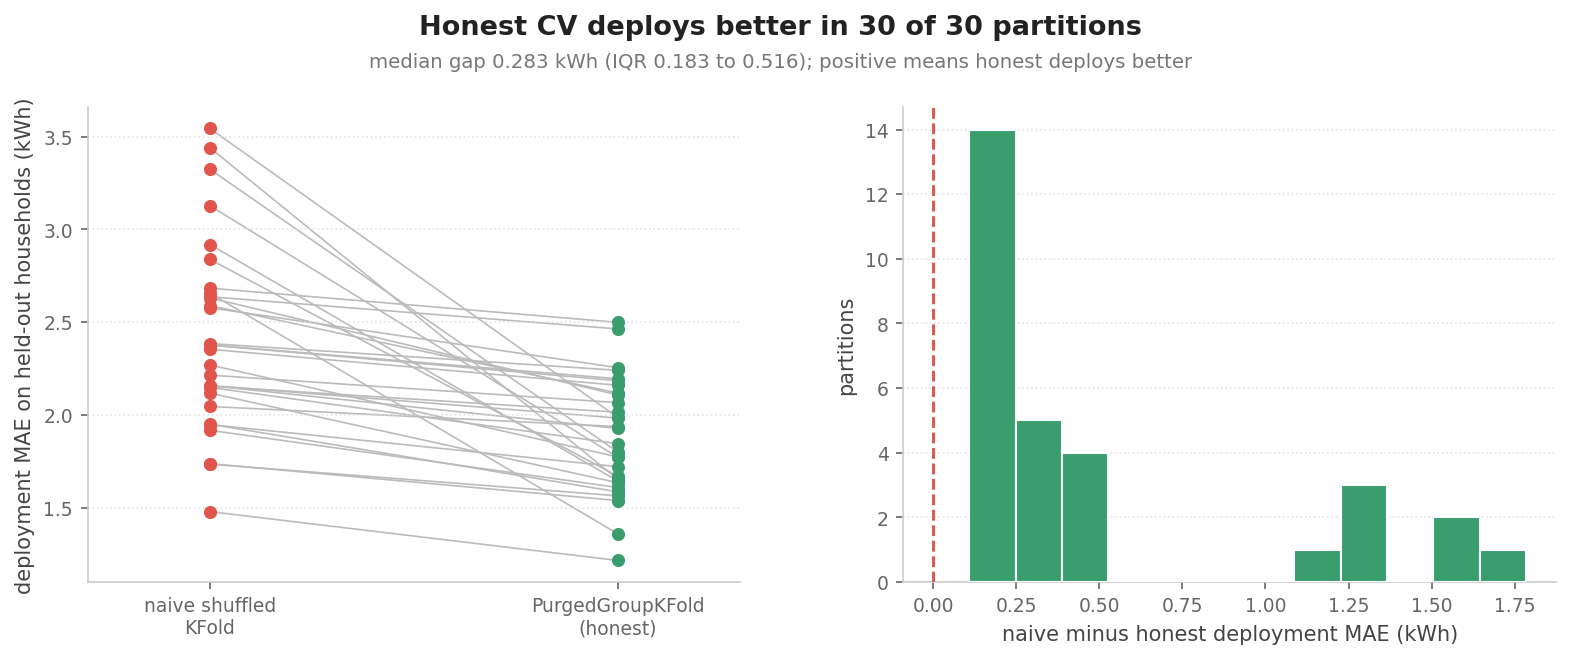
\includegraphics[width=\textwidth]{figures/selection_regret_lcl_seeds.png}
\caption{Left: deployment mean absolute error for the naive and honest selections
in each of the 30 partitions; every paired line falls. Right: distribution of the
naive minus honest deployment-error gap; all of the mass is positive, meaning the
honest selection deploys better in every partition.}
\label{fig:robust}
\end{figure}

\subsection{Removing the identifier erases the gap}

When the household identifier \code{hh_int} is removed from the feature set, both
schemes select Ridge with $\alpha = 0.01$, and both deploy at the same mean
absolute error of 2.4676 kWh on the held-out households. The regret difference
falls to zero. This pins the mechanism precisely: the gap was not a property of
Random Forests in general, nor of the cross-validation arithmetic, but of one
entity-identifier feature that shuffled cross-validation allowed a flexible model
to memorize. Group-aware cross-validation refuses that information during
selection, and the selection then matches what deployment will look like.

\subsection{An innocent, best-practice feature reproduces the effect}

A reviewer may object that a skilled practitioner would never feed a raw
identifier to a tree, so the gap could be an artifact of a contrived feature. The
innocent-feature variant answers this. Replacing the identifier with a
leakage-aware target-mean encoding of the household, the customer's average daily
consumption built per fold with cold-start imputation, reproduces the result. The
gap is larger, not smaller. Across the 30 partitions, naive cross-validation again
selects the unconstrained Random Forest in all 30, while group-aware
cross-validation selects Ridge in 29 and the shallow Random Forest once. The
honest selector picks the best-deploying candidate in all 30 partitions, so its
regret is exactly zero throughout; the naive selector's regret has a median of
0.3645 kWh (interquartile range 0.2998 to 0.4285). The honest selection deploys better
in all 30 partitions, with a median gap of 0.3645 kWh (range 0.1754 to 0.8028)
and a median relative reduction of 15.6\%. On the seed-0 partition the naive
Random Forest deploys at 3.1048 kWh and the honest Ridge at 2.5011 kWh, a gap of
0.6038 kWh. The mechanism is therefore not specific to a raw identifier: any
feature that encodes entity identity, even one engineered with correct per-fold
hygiene, leaks under shuffled folds because the entity sits on both sides of the
split, and the leak is invisible to the cross-validation score that selects the
model.

\subsection{Household structure carries a large generalization penalty at scale}
\label{subsec:population}

The single-grid study above uses one fixed 60-household sample. A full-population
benchmark on the same corpus confirms that the household structure carries a
substantial generalization penalty well beyond that sample, and it does so with
genuinely independent subsamples, which the 30 partitions deliberately are not.
Scanning 167{,}932{,}474 raw rows and drawing 20 independent seeded subsamples of
60 households each from the 4{,}284 eligible households, scoring on entirely
unseen households is 6.03\% worse in weighted absolute percentage error (WAPE,
not the MAE used above) than a pooled temporal estimate (95\% confidence interval
4.93\% to 7.12\%), whereas the purely temporal leakage gap is only 1.60\%. The
estimator there is a single gradient-boosted model rather than a selection grid,
so the two studies are complementary rather than directly comparable; what they
share is the conclusion that the dominant operational risk in this corpus is
household generalization rather than temporal leakage, which is exactly the risk
that group-aware selection is built to measure.

\section{Discussion}

The result has a simple cause. Shuffled cross-validation lets a model see, during
scoring, information it will not have at deployment time, namely the identity and
baseline level of households that will also appear in the test fold. A deep
Random Forest exploits this by learning per-household leaf values, which makes its
cross-validation error look the best in the grid. On households it has never seen,
the identifier is meaningless and the memorized structure is dead weight, so the
deep forest falls behind a regularized linear model. Group-aware cross-validation
removes the leaked information during selection, so its ranking reflects the
deployment condition and it selects the model that actually generalizes.

\citet{teodorescu2025regret} conclude that on independent and identically
distributed tabular data the train and test split dominates regret variance, so
more elaborate cross-validation buys little on average. Our finding is not a
contradiction but a complement that depends on the data regime. On their i.i.d.
data the regret source is largely irreducible. On grouped, time-indexed data the
regret source is reducible: it is entity leakage, and a validation scheme matched
to the deployment unit removes it. We also answer their explicit open question.
They observe that decisions between model \emph{classes} taken on
cross-validation performance are often wrong and call for further investigation;
here the cross-class decision (Ridge versus Random Forest) is wrong under naive
cross-validation in every one of 30 partitions, while under group-aware
cross-validation the chosen model deploys better than the naive choice in all 30
and is at or near the deployment optimum.

This is the leakage that \citet{kapoor2023leakage} and \citet{roberts2021pitfalls}
identify as a recurrent cause of irreproducible models, here in its
entity-leakage form on panel data and traced to its effect on \emph{selection}
rather than on the reported score alone. That load models generalize poorly to
unseen households is itself established \citep{pirbazari2020generalization}. What
we add is that the standard validation default actively rewards the model that
generalizes worst, and that a group-aware split repairs the selection.
We expect the same pattern wherever a repeated-entity panel is validated by
shuffled folds, for example patients, devices, stores, or sensors, although we
have demonstrated it on one dataset and treat that broader claim as a hypothesis
rather than an established result.

The actionable rule is to match the cross-validation unit to the deployment unit.
If a demand forecaster will serve customers who were present during training, a
pooled or temporal split may be appropriate. If it will serve new customers,
selection must hold out customers, because that is the question deployment will
ask. The choice is not a tuning detail; it determines which model class is
shipped. The \pcv{} package makes the group-aware split a drop-in
\pkg{scikit-learn} cross-validator, so adopting the honest selection costs one
line of code.

The study uses one dataset, one forecasting target at daily resolution, and a
deliberately compact grid; the magnitudes will differ on other corpora, horizons,
and richer grids, and a fuller study would sweep these axes. The household
identifier is an intentional and deliberately simple trap. A skilled practitioner
would not feed a raw identifier to a tree, and to that extent the specific
feature is artificial; the defensible claim is the general one, that any
entity-correlated feature opens the same route and that shuffled cross-validation
gives no warning when it does. The ablation confirms this by erasing the gap once
the feature is removed, and the innocent-feature variant confirms it from the
other side: a leakage-aware target encoding of the customer's average load, a
feature a careful practitioner would use, reproduces the gap rather than removing
it. The robustness sweep covers 30 partitions of a single 60-household sample; as
noted, these are correlated resamples, so the descriptive spreads are not
population confidence intervals, and the independent-subsample benchmark uses a
different metric and estimator. Finally, group-aware validation addresses entity
leakage; it does not by itself remove other leakage routes such as globally fit
preprocessing or future-looking feature engineering.

\section{Conclusions}

On a real, partially predictable demand-forecasting task, the cross-validation
scheme used for model selection decided which model class was deployed. Naive
shuffled k-fold consistently selected an unconstrained Random Forest that
memorized household identity and deployed worse on new households, while
group-aware purged cross-validation consistently selected Ridge and deployed
better, by 6.6\% on the headline split and in every one of 30 random partitions.
The effect is removable, not irreducible: it is entity leakage, and a validation
unit matched to the deployment unit removes it. For demand forecasting aimed at
new customers, and for panel forecasting more broadly, validation should be
performed at the granularity of the entity the model will actually face.

\vspace{6pt}

\supplementary{The following supporting information is provided with this article:
the per-partition selection-regret results \path{selection_regret_lcl_seeds.csv}
(main experiment) and \path{selection_regret_lcl_targetenc.csv} (innocent-feature
variant), and the full-population benchmark summary
\path{lcl_full_benchmark_summary.md}.}

\authorcontributions{Conceptualization, methodology, software, validation, formal
analysis, investigation, data curation, writing---original draft, writing---review
and editing, and visualization were all carried out by E.L. The author has read
and agreed to the published version of the manuscript.}

\funding{This research received no external funding.}

\institutionalreview{Not applicable.}

\informedconsent{Not applicable.}

\dataavailability{The Low Carbon London smart-meter data are publicly available
from UK Power Networks and the London Datastore \citep{ukpn_lcl}. The
cross-validation splitter is provided by the open-source \pcv{} package, available
at \url{https://github.com/eslazarev/purged-cross-validation} and on PyPI as
\pkg{purgedcv} \citep{purgedcv2026}; the software is MIT licensed and archived on
Zenodo with DOI \doi{10.5281/zenodo.20312695}. The repository contains the
experiment scripts and notebook that regenerate every reported number and figure
from the public data: \path{examples/selection_regret_lcl_seeds.py}, the
innocent-feature variant \path{examples/selection_regret_lcl_targetenc.py}, and
the single-seed walk-through \path{examples/selection_regret_lcl.ipynb}. The cached
60-household extract (about 68~MB) and the derived seed-level result files are not
redistributed in the repository owing to size; they are regenerated by these
scripts from the public dataset, and the small derived result tables are provided
as Supplementary Materials.}

\acknowledgments{During the preparation of this manuscript the author used OpenAI
Codex and ChatGPT (GPT-5 family) and Anthropic Claude (Claude 4 family) for code
review, refactoring suggestions, and copy-editing. The author has reviewed and
edited the output and takes full responsibility for the content of this
publication; no numerical claim was accepted without executable verification
against the experiment script.}

\conflictsofinterest{The author declares no conflicts of interest.}

%=================================================================
\reftitle{References}

\bibliography{paper}

\end{document}
